\subsection[L'ABC]{L'ABC}

\begin{frame}
	
	\frametitle{Apprendimento supervisionato: ripasso}
	
	\begin{block}{Apprendimento supervisionato}
		Ricordiamo che nell'apprendimento supervisionato si parte da un dataset etichettato (labeled), da quale si cerca di indurre una regola generale per riuscire ad etichettare un nuovo dataset sprovvisto di etichette (unlabeled).
		\newlinedouble
		Nel caso sia possibile effettuare una buona \textit{generalizzazione} possiamo quindi utilizzare il nostro modello di apprendimento supervisionato per prevedere etichette per dei nuovi dati.
		\newlinedouble
		Di seguito di nuovo due immagini riassuntive del funzionamento di un semplice modello ad apprendimento supervisionato.
	\end{block}

\end{frame}



\begin{frame}
	
	\frametitle{Ripasso dal Glossario}
	\framesubtitle{introduciamo alcuni termini ricorrenti nel \ml}
	
	\begin{block}{Modello (il caso classico dell'apprendimento supervisionato)}
		\begin{figure}[!htbp]
			\centering
			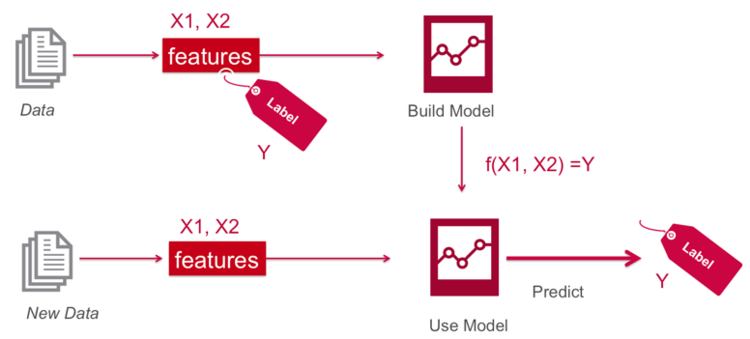
\includegraphics[width=12cm]{images/glossary/supervised_learning_1.png}
			%\caption{Stripe Radar for Fraud Detection}
		\end{figure}
		
	\end{block}

\end{frame}


\begin{frame}
	
	\frametitle{Ripasso dal Glossario}
	\framesubtitle{introduciamo alcuni termini ricorrenti nel \ml}
	
	\begin{block}{Modello (il caso classico dell'apprendimento supervisionato)}
		\begin{figure}[!htbp]
			\centering
			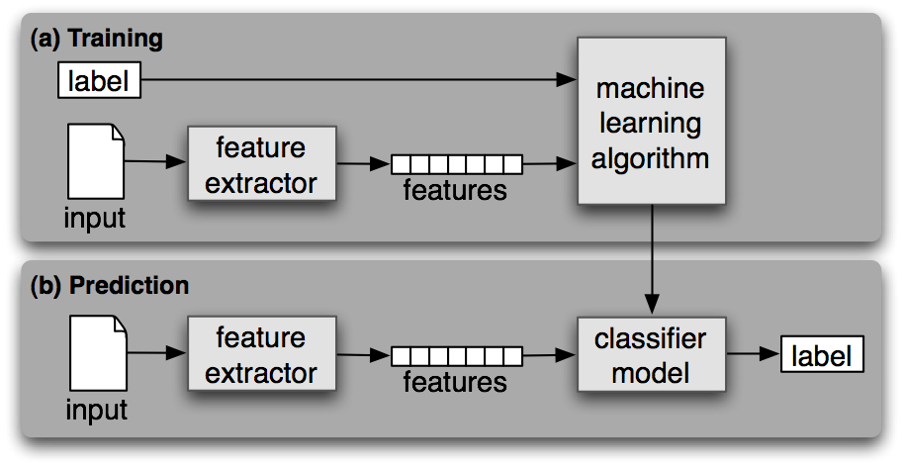
\includegraphics[width=11.2cm]{images/glossary/supervised_learning_2.png}
			%\caption{Stripe Radar for Fraud Detection}
		\end{figure}
		
	\end{block}

\end{frame}
